\documentclass{article}
\usepackage[utf8]{inputenc}
\usepackage{graphicx}
\usepackage{caption}
\usepackage{amsmath}
\usepackage{amssymb}
\usepackage[a4paper, margin=2cm]{geometry}  % <--- Aggiunto per ridurre i bordi
\title{Algebra Lineare}
\author{Nicolò Giuliani}
\date{\today}

\begin{document}
\maketitle
\section{Cosa è un vettore?}
Un \textit{vettore} puo essere visto sia come un oggetto con una lunghezza (modulo) sia una direzione nello spazio.
Graficamente un vettore è rappresentato tramite una freccia.
\\Un vettore in n-dimensioni si scrive come: $\vec{v}=\{v_1,v_2,\text{ }\dots\text{ },v_n\}$.

\begin{figure}[ht]
  \centering
  \begin{minipage}{0.45\textwidth}  % Imposta la larghezza per il testo
    I vettori sono rappresentati tramite una freccia posizionata al di sopra della lettera, lo spostamento quindi si denota come \( \vec{x} \).
    La lunghezza, o meglio modulo, viene indicata attraverso il simbolo del valore assoluto, quindi come \( |\vec{x}|\).
  \end{minipage}
  \begin{minipage}{0.5\textwidth}  % Imposta la larghezza per l'immagine
    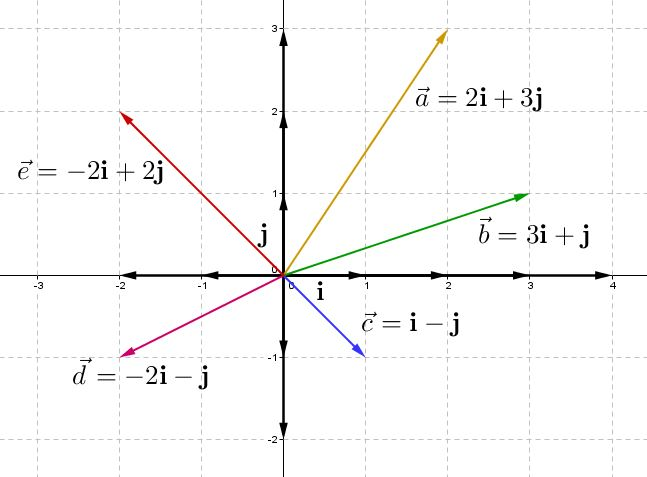
\includegraphics[width=\textwidth]{img/vettori1.jpg}  % Specifica il percorso dell'immagine
    \caption{Diversi vettori in coordinate cartesiane}  % Didascalia sotto l'immagine
    \label{fig:esempio_vettori}
  \end{minipage}
\end{figure}


\par Vediamo ora quali operazioni possiamo fare con i vettori. Quando lavoriamo con essi i numeri ordinari prendono il nome di \textit{scalari}. Quando moltiplichiamo uno scalare con un vettore significa moltiplicare il modulo e cambiare la direzione del vettore.

\begin{figure}[ht]
  \centering
  \begin{minipage}{0.45\textwidth}
    Per esempio, \(-2\vec{x}\) vuol dire avere un vettore lungo il doppio di \(\vec{x}\), ma che punta dalla direzione opposta.
    I vettori possono essere pure sommati, per esempio \(\vec{a} + \vec{b}\) significa disporre l'inizio del vettore \(\vec{b}\) sulla fine di \(\vec{a}\). 
  \end{minipage}
  \begin{minipage}{0.5\textwidth} 
    \centering
    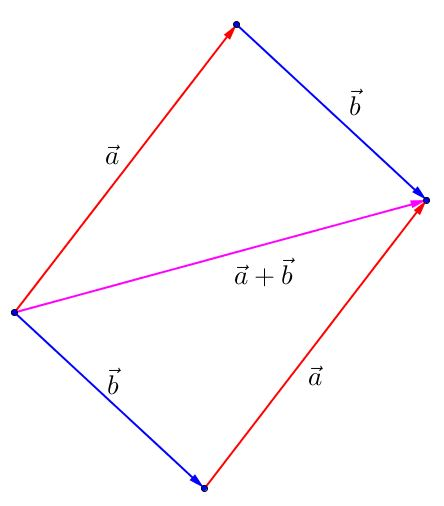
\includegraphics[width=0.8\textwidth]{img/somma.jpg}
    \caption{Somma di vettori}
    \label{fig:somma}
  \end{minipage}
\end{figure}

\par\vspace{20em}  % spazio dall altro paragrafo
\noindent Ora definiamo 3 vettori con modulo pari a 1 disposti lungo gli assi cardinali, questi sono: \(\hat{e_1}, \hat{e_2}, \hat{e_3}\). Questi sono utili perchè possiamo scrivere un vettore \(\vec{V}\) come \(\vec{V}=v_1\hat{e_1}+v_2\hat{e_2}+v_3\hat{e_3}\). Sono chiamati \textit{componenti} di \(\vec{V}\) le quantità \(V_1,V_2,V_3\). Possiamo scrivere un vettore anche come elenco delle sue componenti, in questo caso (\(V_1,V_2,V_3\)).
\par\vspace{1em} Il modulo può essere calcolato attravero il teorema di pitagora nello spazio tridimensionale. \(|\vec{V}|=\sqrt{v_1^2+v_2^2+v_3^2}\).
\par\vspace{1em} Moltiplicare un vettore con uno scalare \(\alpha\) vuol dire moltiplicare \(\alpha\) con ognuna delle componenti. \(\alpha \vec{V}=(\alpha v_1,\alpha v_2, \alpha v_3)\). 
\vspace{1em} \\Possiamo anche moltiplicare due vettori? Certo si chiama \textit{prodotto scalare}. Per calcolare il prodotto scalare di  \(\vec{A}\cdot\vec{B}\) si scrive: \(\vec{A}\cdot\vec{B}=|\vec{A}||\vec{B}|\cos\theta\) dove \(\theta\) è l'angolo tra i due vettori. Possiamo anche calcolare il prodotto scalare con il prodotto delle componenti: \(\vec{A}\cdot\vec{B}=A_1B_1+A_2B_2+A_3B_3 \). \textit{Ricorda}: se i due vettori sono ortogonali (perpendicolari) il loro prodotto a scalare è nullo.

\pagebreak
\section{Matrici e sistemi lineari}
Consideriamo un \textit{sistema lineare} della forma: 
\begin{equation*}
  \left\{
  \begin{aligned}
    a_{11}x_1 + a_{12}x_2 + \dots + a_{1n}x_n &= b_1 \\
    a_{21}x_1 + a_{22}x_2 + \dots + a_{2n}x_n &= b_2 \\ 
    \quad \vdots \quad \\
    a_{m1}x_1 + a_{m2}x_2 + \dots + a_{mn}x_n &= b_m
  \end{aligned}
  \right.
\end{equation*}
il sistema può essere riscritto utilizzando il prodotto righe per colonne:
\[
\begin{pmatrix}
  a_{11} & a_{12} & \dots{} & a_{1n} \\
  a_{21} & a_{22} & \dots{} & a_{2n} \\
  \vdots{} & \vdots & & \vdots \\
  a_{m1} & a_{m2} & \dots{} & a_{mn}
\end{pmatrix}
\begin{pmatrix}
  x_1 \\
  x_2 \\
  \dots \\
  x_n
\end{pmatrix}
=
\begin{pmatrix}
  b_1 \\
  b_2 \\
  \dot{} \\
  b_m
\end{pmatrix}
\]
o sinteticamente: \(A\vec{x}=\vec{b}\). \\
Dove \(A=(a_{ij})\) è la matrice \textit{$m \times n$} si chiama \textit{matrice incompleta} associata al sistema, mentre: 
\[
(A|\vec{b})=
\left(
\begin{array}{cccc|c}
a_{11} & a_{12} & \dots & a_{1n} & b_1 \\
a_{21} & a_{22} & \dots & a_{2n} & b_2 \\
\vdots & \vdots &  & \vdots & \vdots \\
a_{m1} & a_{m2} & \dots & a_{mn} & b_m
\end{array}
\right)
\]
la definiamo come matrice \textit{completa associata} al sistema. 
\vspace{1em} \\\textbf{Definizione 1.3.2} Una matrice si dice in \textit{forma a scala} (righe), o anche detto \textit{a scala}, se sono soddisfatte le secondi condizioni:
\vspace{10px}\par (a) eventuali righe non nulle si trovano in fondo alla matrice
\vspace{5px}\par (b) il primo elemento non nullo di ogni riga si deve trovare più a destra dell'elemento non nullo della riga precedente, ovvero quella al di sopra.
\vspace{1em} \\\textbf{Definizione 1.3.4} Sia A una matrice a scala (per righe). Si chiama \textit{pivot} di A il primo elemento non nullo di ogni riga di A. Si chiama \textit{rango righe} di A il numero di pivot che una matrice ha, si indica con rr(A).
\vspace{3px}\\ Osservazione: Se A $\in M_{m,n}(\mathbb{R})$ a scala:
\begin{align*}
  rr(A) \leq m \\
  rr(A) \leq n
\end{align*}
\vspace{5px} \\\textbf{Definizione 1.3.7} Il sistema \(A\vec{x}=\vec{b}\) si dice a scala se la matrice A è in forma scalare.
\\ \textbf{Proposizione 1.3.10} Sia \(A\vec{x}=\vec{b}\) un sistema lineare a scala nelle n incognite \(x_1,\dots,x_n\):
\vspace{3px}
\par (a) se $rr(A) = rr(A|\vec{b})$ il sistema ha soluzioni;
\par (b) se $rr(A) = rr(A|\vec{b}) = n$ il sistema a una sola soluzione;
\par (c) se $rr(A) = rr(A|\vec{b}) = k < n$ il sistema ha inifinite soluzioni che dipendono da n-k variabili.
\vspace{1em}
\subsection{Algoritmo di Gauss}
Ipotizziamo di avere un sistema lineare \(A\vec{x}=\vec{b}\) e trasformarlo in un sistema a scala \(A'\vec{x}=\vec{b}'\) con le stesse soluzioni.
\\ \textbf{Definizione 1.4.2} Le \textit{operazioni elementari} sulle righe di A sono:
\vspace{3px}
\par (a) scambio di righe. ($R_i \iff R_j$)
\par (b) moltiplicazione di una riga per un numero reale diverso da 0. (\(R_i \to \alpha R_i \text{ con } \alpha \neq 0, \text{ } \alpha \in \mathbb{R}\))
\par (c) sostituzione della riga \textit{i} con la somma della riga \textit{i} e la riga \textit{j} moltiplicata per un numero reale. ($R_i \to R_i + \alpha R_j \text{ con }  \alpha \in \mathbb{R}$)

\pagebreak
\section{Spazi vettoriali}
Per rappresentare un vettore bisogna utilizzare uno spazio vettoriale, infatti un vettore è un elemento di uno spazio vettoriale.
\\Questo è rappresentato come
\begin{align*}
  \vec{v}=\{v_1,v_2,\text{ }\dots\text{ },v_n\} \in \mathbb{R}^n
\end{align*}
\textbf{Definizione 2.3.1} Si dice \textit{spazio vettoriale} reale un insieme V che gode delle operazioni:
\begin{align*}
  \text{somma: } V \times V \to V \\
  \text{prodotto: } \mathbb{R} \times V \to V
\end{align*}
ovvero
\begin{align*}
  \text{($\vec{u}$,$\vec{v}$)} \to \vec{u}+\vec{v} \\
  \text{($\lambda$, $\vec{u}$)} \to \lambda \vec{u}
\end{align*}

Esempio di spazio vettoriale:
\begin{align*}
  \mathbb{R}^2 = \{(x,y) \mid x,y \in \mathbb{R}\}
\end{align*}
o meglio definito:
\begin{align*}
  \mathbb{R}^n = \{(x_1,\text{ }\dots \text{ }, x_n) \mid x_1,\text{ } \dots \text{ },x_n \in \mathbb{R}\}
\end{align*}
\subsection{Sottospazi vettoriali}
Sia W sottoinsieme di V, si definisce W un \textit{sottospazio vettoriale} a V, ovvero $W \subseteq V$, se:
\vspace{5px}\par (a) $W\neq \emptyset \quad \to \quad 0_V \in W$ ($0_V$ è lo spazio vettoriale costituito solo dal vettore nullo, si chiama \textit{spazio vettoriale banale})
\vspace{3px}\par (b) W è chiuso rispetto la somma. $\forall \vec{u},\vec{v} \in W \to \vec{u} \vec{v} \in W$
\vspace{3px}\par (c) W è chiuso rispetto il prodotto. $\forall \vec{u} \in W \text{ e } \forall \lambda \in \mathbb{R} \to \lambda \vec{u} \in W$

\subsection{Combinazioni lineari e generatori}
Ricapitolando: se $\forall V \neq \emptyset \to \forall \vec{v_i} \in V (i > 0)$  e questo implica che $\forall \lambda \vec{v_i} \in V$ con $\forall \lambda \in \mathbb{R}$. 
\vspace{1px}  \\ In $\mathbb{R}^2$ consideriamo i vettori (1,0) e (0,1). Dobbiamo cercare il più piccolo sottospazio di $\mathbb{R}^2$, chiamiamolo W,  che contenga i due vettori.
\begin{align*}
  (1,0) \in W \to W_1 \in W \text{ con } W_1 = \{\lambda (1,0) \mid \lambda \in \mathbb{R}\} \\
  (0,1) \in W \to W_2 \in W \text{ con } W_2 = \{\mu (0,1) \mid \mu \in \mathbb{R}\} 
\end{align*}
e sappiamo dalla definizione di sottospazio vettoriale anche che la somma di due vettori di W appartiene sempre ad W.
\begin{align*}
  (1,0) \in W \text{ e } (0,1) \in W \iff (1,0)+(0,1)=(1,1) \in W
\end{align*}
e quindi abbiamo
\begin{align*}
  W = \{\lambda(1,0) + \mu(0,1) \mid \lambda,\mu \in \mathbb{R}\}
\end{align*}
che se moltiplichiamo gli scalari otteniamo
\begin{align*}
  W = \{(\lambda,0) + (0,\mu) \mid \lambda,\mu \in \mathbb{R}\}
\end{align*}
ovvero se sommato
\begin{align*}
  W = \{(\lambda, \mu) \mid \lambda,\mu \in \mathbb{R}\} = \mathbb{R}^2
\end{align*}
Questo concetto viene chiamato \textit{generazione} di un sottospazio vettoriale. 
\vspace{1em}
\\
\textbf{Definizione 3.1.1}
\\ Sia:
\begin{align*}
  V = \{ \vec{v_1}, \text{ } \dots \text{ }, \ \vec{v_n} \} 
\end{align*}
\begin{align*}
  w = \{\lambda_1 \vec{v_1}, \text{ } \dots \text{ }, \lambda_n \vec{v_n} \mid \lambda_1, \text{ } \dots \text{ }, \lambda_n \in \mathbb{R}\}
\end{align*}
$w$ si dice \textit{combinazione lineare} di $\vec{v_1}, \text{ } \dots \text{ }, \vec{v_n}$ con scalari $\lambda_1, \text{ } \dots \text{ }, \lambda_n$.
\vspace{1em}
\\
\textbf{Definizione 3.1.2}
\\ Sia: 
\begin{align*}
   \{ \vec{v_1}, \text{ } \dots \text{ }, \ \vec{v_n} \} \subseteq V
\end{align*}
si indica il \textit{sottospazio generato} da $v_1, \text{ } \dots \text{ }, v_n$ con 
\begin{align*}
  \langle \vec{v_1}, \text{ } \dots \text{ }, \vec{v_n} \rangle = \{\lambda_1 \vec{v_1} + \text{ } \dots \text{ } + \lambda_n \vec{v_n} \mid \lambda_1, \text{ } \dots \text{ }, \lambda_n \in \mathbb{R}\}
\end{align*}
si può anche scrivere come $span\{v_1, \text{ } \dots \text{ }, v_n\}$.
\\ Ricapitolando: lo span generato da un vettore non nullo in $\mathbb{R}^2$ corrisponde una retta, mentre il sottospazio generato da due vettori (1,0) e (0,1) genera tutto $\mathbb{R}^2$.
\\ \textbf{Osservazione 3.1.3}
\\ Se V è uno spazio vettoriale e $v \in V$ allora lo span\{v\} è $\langle v \rangle = \{\lambda \mid \lambda \in \mathbb{R}\}$ mentre lo span\{0\} = \{0\}. 

\vspace{5px}
\textbf{\\ Definizione 3.1.4}  
\\ Sia \(V\) uno spazio vettoriale e siano \(v_1, \dots, v_n \in V\).  
Si dice che \(v_1, \dots, v_n\) \textit{generano} \(V\), o anche che \(\{v_1, \dots, v_n\}\) è un \textit{insieme di generatori} di \(V\), se vale \[ V = \langle v_1, \dots, v_n \rangle. \]


\textbf{\\Proposizione 3.1.5}
\\ Sia V uno spazio vettoriale e siano \(v_1, \dots, v_n \in V\).  Allora sappiano che $\langle v_1, \dots, v_n\rangle$ è uno sottospazio di V.  
Inoltre se Z è uno sottospazio di V e \(v_1, \dots, v_n \in Z\) implica che $span\{v_1, \text{ } \dots \text{ }, v_n\} \subseteq Z$, quindi $\langle v_1, \text{ } \dots \text{ }, v_n \rangle$ è il più piccolo sottospazio di V che contiene $v_1, \text{ }\dots\text{ }, v_n$.
\vspace{3px}
\\Dimostrazione:
\begin{align*}
  0 \in span\{v_1, \dots, v_n \} \text{ perchè } 0 = \{0v_1, \text{ } \dots \text{ }, 0v_n\}
\end{align*}
e da qui abbiamo \textit{(a)} della definizione di sottospazio.
\\Siano
\begin{align*}
  v,w \in span\{v_1, \dots, v_n\}
\end{align*}
allora da definizione di combinazione lineare (3.1.2):
\begin{align*}
  v = \{\alpha_1 \vec{v_1}, \text{ }\dots\text{ }, \alpha_n \vec{v_n} \mid \alpha_1, \text{ }\dots\text{ }, \alpha_n \in \mathbb{R}\}
  \\   w = \{\beta_1 \vec{v_1}, \text{ }\dots\text{ }, \beta_n \vec{v_n} \mid \beta_1, \text{ }\dots\text{ }, \beta_n \in \mathbb{R}\}
\end{align*}
e da definizione di spazio vettoriale (2.3.1):
\begin{align*}
  v+w=\{(\alpha_1+\beta_1)\vec{v_1}, \text{ }\dots\text{ }, (\alpha_n+\beta_n)\vec{v_n}\} \in span\{\vec{v_1}, \text{ }\dots\text{ }, \vec{v_n}\}
\end{align*}
e da qui abbiamo \textit{(b)} della definizione di sottospazio.
\\ Inoltre se $k \in \mathbb{R}$
\begin{align*}
  kv=\{(k\alpha_1)\vec{v_1},\text{ }\dots\text{ },(k\alpha_n)\vec{v_n} \in span\{\vec{v_1}, \text{ }\dots\text{ }, \vec{v_n}\}\}
\end{align*}
e infine abbiamo dimostrato anche \textit{(c)} della definizione di sottospazio.
\\Vediamo ora che lo $span\{\vec{v_1}, \text{ }\dots\text{ }, \vec{v_n}\}$ è il piu piccolo sottospazio vettoriale che contiene $\{\vec{v_1}, \text{ }\dots\text{ }, \vec{v_n}\}$.
Sia $v=\{\lambda_1\vec{v_1},\text{ }\dots\text{ },\lambda_n\vec{v_n} \mid \lambda_1,\text{ }\dots\text{ },\lambda_n\in \mathbb{R} \} \in span\{\vec{v_1},\text{ }\dots\text{ },\vec{v_n}\}$.
Inoltre $\vec{v_1},\text{ }\dots\text{ },\vec{v_n} \in Z$, che è uno sottospazio di V, allora $\lambda_1\vec{v_1},\text{ }\dots\text{ },\lambda_n\vec{v_n} \in Z$, da definizione di sottospazio vettoriale. Quindi $v\in Z$, allora $span\{\vec{v_1},\text{ }\dots\text{ },\vec{v_n}\} \subseteq Z$.

\vspace{1em}
\textbf{\\Proposizione 3.1.8}
\\ Sia V uno spazio vettoriale e $\vec{v_1},\text{ }\dots\text{ },\vec{v_n} \in V$ e w una \textit{combinazione lineare} di $\vec{v_1},\text{ }\dots\text{ },\vec{v_n}$, cioè $w=\{\lambda_1\vec{v_1},\text{ }\dots\text{ },\lambda_n\vec{v_n}\mid\lambda_1,\text{ }\dots\text{ },\lambda_n \in \mathbb{R}\}$.
\\ Allora
\begin{align*}
  span\{\vec{v_1},\text{ }\dots\text{ },\vec{v_n}\} \subseteq span\{\vec{v_1},\text{ }\dots\text{ },\vec{v_n},w\} \iff span\{\vec{v_1},\text{ }\dots\text{ },\vec{v_n}\} = span\{\vec{v_1},\text{ }\dots\text{ },\vec{v_n},w\}
\end{align*}
La dimostrazione è basata sulla proposizione 3.1.5.

\pagebreak
\subsection{Indipendenza lineare}
Sia V uno spazio vettoriale. 
I vettori $\vec{v_1},\text{ }\dots\text{ },\vec{v_n} \in V$ si dicono \textit{linearmente indipendenti} se
\begin{align*}
  \lambda_1\vec{v_1}+\text{ }\dots\text{ }+\lambda_n\vec{v_n} = 0
\end{align*}
se
\begin{align*}
  \lambda_1=\text{ }\dots\text{ }=\lambda_n=0
\end{align*}
Anche $\{\vec{v_1},\text{ }\dots\text{ },\vec{v_n}\}$ si dice linearmente indipendente.
\\ Al contrario se abbiamo $\lambda_1,\text{ }\dots\text{ },\lambda_n$ non nulli l'insieme $\{\vec{v_1},\text{ }\dots\text{ },\vec{v_n}\}$ si dice \textit{linearmente dipendente}.

\vspace{5px}
\textbf{\\Osservazione 3.2.3}
\\ Se in un insieme di vettori c'è il vettore nullo allora questo sarà sempre linearmente dipendente.
\begin{align*}
  \{\vec{v_1}=0,\text{ }\dots\text{ },\vec{v_n}\} \to 1\vec{v_1}+\text{ }\dots\text{ }+0\vec{v_n}=0
\end{align*}
ma da definizione di indipendenza lineare $\lambda_1\neq0$, quindi si ha un insieme linearmente dipendente.
\vspace{5px}
\textbf{\\Proposizione 3.2.4}
\\ In uno spazio vettoriale V, i vettori $\vec{v_1},\text{ }\dots\text{ },\vec{v_n}$ sono linearmente dipendenti se almeno un vettore è combinazione lineare di un'altro.
\vspace{5px}
\textbf{\\Proposizione 3.2.5}
\\ Se due vettori non sono multipli uno dell'altro implica che questi sono linearmente indipendenti. Non vale però il contrario, ovvero non è detto che se sono multipli questi siano linearmente dipendenti.
\vspace{5px}
\textbf{\\Proposizione 3.2.8}
\\ Un sottoinsieme non vuoto di un insieme formato da vettori linearmente indipendenti è formato da vettori linearmente indipendenti.

\pagebreak
\section{Basi e dimensioni}
Una base serve per ricostruire uno spazio vettoriale con meno vettori possibili.
\\Per esempio possiamo generare $\mathbb{R}^2$ dall'insieme $\{(1,0),(0,1)\}$ che è linearmente indipendente mentre l'insieme $\{(1,0),(0,1),(1,1)\}$, genera comunque ma, è linearmente dipendente.
Quindi possiamo eliminare dal secondo generatore il vettore (1,1) e ottenere un generatore dove nessun vettore è combinazione lineare degli altri.
\\ Questo vuol dire che se eliminiamo da un generatore tutti i vettori che sono combinazione lineare di un'altro vettore otterremo un generatore con vettori linearmente indipendenti.

\vspace{5px}
\textbf{\\Proposizione 4.1.2}
\\Sia $V=\langle\vec{v_1},\text{ }\dots\text{ },\vec{v_n}\rangle \neq \{0\}$. Allora esiste un sottoinsieme linearmente indipendente che genera sempre V.

\vspace{5px}
\textbf{\\Proposizione 4.1.3}
\\Sia V uno spazio vettoriale. $\langle \vec{v_1},\text{ }\dots\text{ },\vec{v_n}\rangle$ si dice \textit{base} se:
\vspace{2px}\\ 1) I vettori $\langle \vec{v_1},\text{ }\dots\text{ },\vec{v_n}\rangle$ sono linearmente indipendenti.
\vspace{2px}\\ 2) I vettori $\langle \vec{v_1},\text{ }\dots\text{ },\vec{v_n}\rangle$ generano V.

\vspace{5px}
\textbf{\\Teorema 4.1.4}
\\ Siano $\langle \vec{v_1},\text{ }\dots\text{ },\vec{v_n}\rangle$ vettori in uno spazio vettoriale V.
\vspace{2px}\\ 1) $\langle \vec{v_1},\text{ }\dots\text{ },\vec{v_n}\rangle$ è una base di V solo se è un insieme minimale composto da generatori di V.
\vspace{2px}\\ 2) $\langle \vec{v_1},\text{ }\dots\text{ },\vec{v_n}\rangle$  è una base di V solo se è un insieme massimale composto da vettori linearmente indipendenti.

\vspace{5px}
\textbf{\\Proposizione 4.1.6}
\\ Se uno spazio vettoriale $V \neq \{0\}$ è generato da un numero finito di vettori $\vec{v_1},\text{ }\dots\text{ }\vec{v_n}$, allora esiste una base di V.

\vspace{5px}
\subsection{Dimensione}
Tutte le basi di uno spazio vettoriale hanno un numero fisso di elementi, queso numero si dice \textit{dimensione} dello spazio vettoriale.

\textbf{\\ Teorema del completamento 4.2.1}
\\Sia V uno spazio vettoriale finitamente generato, $\{\vec{v_1},\text{ }\dots\text{ },\vec{v_m}\} \subseteq V$ e che $\{\vec{v_1},\text{ }\dots\text{ },\vec{v_m}\}$ sia linearmente indipendente. Se $\beta=\{\vec{w_1},\text{ }\dots\text{ },\vec{w_n}\}$ è una base di V. Allora $m \leq n$ e possiamo aggiungere al insieme $\{\vec{v_1},\text{ }\dots\text{ },\vec{v_m}\}$ n-m vettori di $\beta$ per ottenere una base di V.
\vspace{8px}
\textbf{\\Proposizione 4.2.3}
\\Il numero di elementi di una base di uno spazio vettoriale V si chiama \textit{dimensione} e si indica con $dim(V)$. Quando V è generato da una base con elementi finiti si dice \textit{dimensione finita}.
\vspace{2px}\\Basi canoniche:
\begin{align*}
  \text{1) }\mathbb{R}^n \to C =\{\vec{e_1},\text{ }\dots\text{ },\vec{e_n}\} 
\end{align*}
\\con $\vec{e_i}$ che ha nella cordinata $i$ valore 1, mentre nelle altre ha il valore 0.
\\Per esempio: $\mathbb{R}^3 \text{ ha come base canonica } C=\{(1,0,0),(0,1,0),(0,0,1)\}$.
\begin{equation*}
  \text{2) }\mathbb{R}_n[x] \to C=\{x^n,x^{n-1},\text{ }\dots\text{ },x,1\}
\end{equation*}
ovvero lo spazio vettoriale dei polinomi di grado massimo $n$.
\begin{equation*}
  \text{3) }M_{m,n} \to C=\{E_{1,1},\text{ }\dots\text{ },E_{m,n}\}
\end{equation*}
\\ovvero $E_{i,j}$ ha come valore 1 nella posizione $(i,j)$ e ha 0 nelle altre posizioni.
\\Per esempio la base canonica di $M_{2,3}$:
\begin{align*}
  C = \{
    \begin{pmatrix}
    1 & 0 & 0 \\
    0 & 0 & 0
  \end{pmatrix},
  \begin{pmatrix}
    0 & 1 & 0 \\
    0 & 0 & 0
  \end{pmatrix},
  \begin{pmatrix}
    0 & 0 & 1 \\
    0 & 0 & 0
  \end{pmatrix},
  \begin{pmatrix}
    0 & 0 & 0 \\
    1 & 0 & 0
  \end{pmatrix},
  \begin{pmatrix}
    0 & 0 & 0 \\
    0 & 1 & 0
  \end{pmatrix},
  \begin{pmatrix}
    0 & 0 & 0 \\
    0 & 0 & 1
  \end{pmatrix}
  \}
\end{align*}

Quindi ricapitolando:
\begin{align*}
  \text{1) }dim(\mathbb{R}^n)=n \\
  \text{2) }dim(\mathbb{R}_n[x])=n+1 \\
  \text{3) }dim(M_{m,n})=mn
\end{align*}

\vspace{5px}
\textbf{\\Proposizione 4.2.4}
\\ Sia V uno spazio vettoriale e W un suo sottospazio vettoriale:
\begin{align*}
  \text{1) }dim\{W\} \leq dim\{V\} \\
\end{align*}
\begin{align*}
  \text{2) }dim\{W\} = dim\{V\} \iff V=W
\end{align*}
\vspace{5px}
\textbf{\\Proposizione 4.2.6}
\\ Sia V uno spazio vettoriale, $dim\{V\}=n$ e $\{\vec{v_1},\text{ }\dots\text{ },\vec{v_n}\} \subseteq V$. 
\\Allora le seguenti frasi sono equivalenti: 
\\\\
a) $\{\vec{v_1},\text{ }\dots \text{ },\vec{v_n}\}$ è una base di V. \\
b) $\vec{v_1},\text{ }\dots\text{ },\vec{v_n}$ sono linearmente indipendenti. \\
c) $\vec{v_1},\text{ }\dots\text{ },\vec{v_n}$ generano V. \\

\pagebreak
\textbf{\\Teorema 4.2.8}
\\ Sia $\beta=\{\vec{v_1},\text{ }\dots\text{ },\vec{v_n}\}$ una \textit{base ordinata} per lo spazio vettoriale V. Sia $v \in V$. Allora esiste unicamente la tupla di lunghezza $n$ composta dagli scalari $(\alpha_1,\text{ }\dots\text{ },\alpha_n)$ tale che:
\begin{align*}
  v=\{\alpha_1\vec{v_1},\text{ }\dots\text{},\alpha_n\vec{v_n}\}
\end{align*}

\textbf{\\Definizione 4.2.9}
\\Gli scalari $(\alpha_1,\text{ }\dots\text{ },\alpha_n)$ del Toerema precedente si chiamano \textit{componenti} di $v \in V$ nella base $\beta$ o anche \textit{cordinate} di $v$ rispetto alla base $\beta$. Vengono indicate con $(v)_\beta=(\alpha_1,\text{ }\dots\text{ },\alpha_n)$.

\vspace{10px}
\subsection{Algoritmo di Gauss applicato in modo diretto}
Data una matrice $A \in M_{m,n}(\mathbb{R})$ ogni sua riga può essere considerato un vettore di $\mathbb{R}^n$.
\textbf{\\Proposizione 4.3.1} \\Data una matrice $A \in M_{m,n}(\mathbb{R})$ le operazioni di Gauss non cambiano il sottospazio generato dai vettori riga di A.
\textbf{\\Proposizione 4.3.3} \\Se una matrice A è a scala i suoi vettori non nulli sono linearmente indipendenti.
\vspace{1em}
\\Istruzioni per applicare l'algoritmo in modo diretto:
\\1) Scriviamo la matrice $A \in M_{k,n}(\mathbb{R})$ che ha come vettori $\vec{v_1},\text{ }\dots\text{ },\vec{v_k}$.
\\2) Otteniamo una nuova matrice $A'$ a scala da A.
\\3) I vettori non nulli generano un sottospazio $W$ e sono linearmente indipendenti (4.3.3), quindi generano $W$.
\\4) Sia $r$ il $rr(A')$, ovvero il numero di pivot o meglio il numero di righe non nulle di $A'$; quindi $dim(W)=r$. Se $k$ (numero di righe) $=r$, i vettori $\vec{v_1},\text{ }\dots\text{ },\vec{v_k}$ generano uno spazio di dimensione $k$. invece se $k>r$ i vettori sono linearmente dipendenti.
\vspace{15px}
\\Vediamo ora come ottenere una base di un sottospazio $W \subset \mathbb{R}^n$ e completarla ad una base di $\mathbb{R}^n$:
\\1) Scriviamo la matrice che ha come vettori $\vec{w_1},\text{}\dots\text{ },\vec{w_k}$.
\\2) Usiamo Gauss per ottenere una matrice $A'$ a scala per righe.
\\3) $r=rr(A')$ e gli r-vettori, non nulli, generano $W$. Questi sono linearmente indipendenti e sono una base di W.
\\4) Per completare la base ad una base di $\mathbb{R}^n$ basta aggiungere $n-r$ vettori riga nelle posizioni mancanti nella matrice a scala. Così otteniamo una nuova matrice $A''$ a scala con $n$ pivot. Da 4.3.3 sappiano che i vettori sono linearmente indipendenti e dato che $dim{\mathbb{R}^n}=n$ per 4.2.6 gli $n$ vettori sono base di $\mathbb{R}^n$.

\pagebreak
\section{Applicazioni lineari}
Le applicazioni lineare sono funzioni tra gli spazi vettoriali, essi rispettano le stesse proprieta delle operazioni come somma e moltiplicazione. Questi sono rappresentati attraverso le matrici.
\\ In analisi le funzioni associano un insieme di partenza  detto \textit{dominio} ad uno di arrivo chiamato \textit{codominio}.
\\ Per esempio $f : \mathbb{R} \to \mathbb{R}$, con $f(x)=x^2$. Essa è una funzione da $\mathbb{R}$ a $\mathbb{R}$. Come sappiamo $\mathbb{R}$ è uno spazio vettoriale, quindi f è una funzione di uno spazio vettoriale che parte da $\mathbb{R}$ a $\mathbb{R}$.
\\ Vengono chiamate \textit{applicazioni lineari} le funzioni  che rispettano la struttura degli spazio vettoriali.

\vspace{5px}
\textbf{\\Definizione 5.1.1}
\\Definiamo una funzione $f$ tra due insiemi $A$ e $B$, dove per ogni elemento di $A$ si collega ad un singolo elemento di $B$.
\begin{align*}
  f : A \to B \\
   a \to f(a)
\end{align*}
L'insieme $A$ è detto \textit{dominio} della funzione, mentre l'insieme B si dice \textit{codominio}.
\\L'\textit{immagine} gli elementi di $f(a)$ in B. Ovvero:  $\forall a \in A \to f(a) \in B$, questo si indica con $Im(f)$.
\vspace{5px}
\textbf{\\Definizione 5.1.2}
\\ Siano V e W due spazi vettoriali e sia $F : V \to W$ una funzione, questa viene chiamata \textit{applicazione lineare} se:
\begin{align}
  F(u+v)=F(u)+F(v) \mid \forall u,v \in V \\
  F(\lambda u)=\lambda F(u) \mid \forall \lambda \in \mathbb{R}, \forall u \in V
\end{align}
quindi si può riassumere in
\begin{align*}
  F(\lambda u + \mu v)= \lambda F(u)+ \mu F(v) \mid \forall \lambda,\mu \in \mathbb{R}, \forall u,v \in V
\end{align*}

\pagebreak
\textbf{\\Osservazione 5.1.6}
\\ A ogni matrice
\begin{align*}
  A=\begin{pmatrix}
    a_{11} & a_{12} & \dots & a_{1n} \\
    a_{21} & a_{22} & \dots & a_{2n} \\
    \vdots & \vdots & & \vdots \\
    a_{m1} & a_{m2} & \dots & a_{mn} 
  \end{pmatrix} \in M_{m,n}(\mathbb{R})
\end{align*}
possiamo associare la funzione $L_A : \mathbb{R}^n \to \mathbb{R}^m$
\begin{align*}
  L_A : 
  \mathbb{R}^n 
  \begin{pmatrix}
    x_1 \\
    x_2 \\
    \vdots \\
    x_n
  \end{pmatrix}
  \to 
  \mathbb{R}^m 
  \begin{pmatrix}
    a_{11}x_1 + a_{12}x_2+\dots+a_{1n}x_n \\
    a_{21}x_1 + a_{22}x_2+\dots+a_{2n}x_n \\
    \vdots \\
    a_{m1}x_1 + a_{m2}x_2+\dots+a_{mn}x_n
  \end{pmatrix}
  = \begin{pmatrix}
    a_{11} & a_{12} & \dots & a_{1n} \\
    a_{21} & a_{22} & \dots & a_{2n} \\
    \vdots & \vdots && \vdots \\
    a_{m1} & a_{m2} & \dots & a_{mn}
  \end{pmatrix}
  \begin{pmatrix}
    x_1 \\
    x_2 \\
    \vdots \\
    x_n
  \end{pmatrix}
  =
  A\begin{pmatrix}
    x_1 \\
    x_2 \\
    \vdots \\
    x_n
  \end{pmatrix}
\end{align*}
Per esempio:
\begin{align*}
  A=\begin{pmatrix}
    2 & 1 & 0 \\
    -1 & 1 & 3
  \end{pmatrix}
\end{align*}
Si ha che $L_A : \mathbb{R}^3 \to \mathbb{R}^2$
\begin{align*}
  L_A\begin{pmatrix}
    x_1 \\
    x_2 \\
    x_3
  \end{pmatrix}
  =
  \begin{pmatrix}
    2 & 1 & 0\\
    -1 & 1 & 3
  \end{pmatrix}
  \begin{pmatrix}
    x_1 \\
    x_2 \\
    x_3
  \end{pmatrix}
  =
  \begin{pmatrix}
    2x_1+x_2 \\
    -x_1+x_2+3x_3
  \end{pmatrix}
  = 
  x_1\begin{pmatrix}
    2 \\
    -1
  \end{pmatrix}
  +x_2\begin{pmatrix}
    1 \\
    1
  \end{pmatrix}
  +x_3\begin{pmatrix}
    0 \\
    3
  \end{pmatrix}
\end{align*}
Così si può ottenere le immagini dei vettori della base canonica:
\begin{align*}
  L_A\begin{pmatrix}
    1 \\ 0 \\ 0
  \end{pmatrix}
  =
  \begin{pmatrix}
    2 \\ -1
  \end{pmatrix}
  \qquad
  L_A\begin{pmatrix}
  0 \\ 1 \\ 0
  \end{pmatrix}
  =
  \begin{pmatrix}
    1 \\ -1
  \end{pmatrix}
  \qquad
  L_A\begin{pmatrix}
    0 \\ 0 \\ 1
    \end{pmatrix}
    =
    \begin{pmatrix}
      0 \\ 3
    \end{pmatrix}
\end{align*}
Come deve essere fatta una funzione $F : \mathbb{R} \to \mathbb{R}$ per essere \textit{lineare}?
\\Sia $F(1)=\alpha \in \mathbb{R}$, sappiamo quindi che $F(x)=xF(1)=\alpha x$. Quindi le applicazioni lineari da $\mathbb{R}\to\mathbb{R}$ hanno come grafico una retta che passa per l'origine.

\vspace{5px}
\textbf{\\Teorema 5.1.7}
\\Siano V e W due spazi vettoriali. Se $\{\vec{v_1},\text{ }\dots\text{ },\vec{v_n}\}$ è una base di V e $\vec{w_1},\text{ }\dots\text{ },\vec{w_n} \in W$, non per forza $\vec{v_i}\neq\vec{w_i}$. Allora esiste una unica applicazione lineare $L : V \to W$ tale che
\begin{align*}
  L(v_1)=w_1;\\
  \\
  L(v_n)=w_n;
\end{align*}
\vspace{5px}
\textbf{\\Corollorio 5.1.8}
\\Siano V e W due spazi vettoriali, se due applicazioni lineare $T,S:V \to W$ condicono su una base di V allora concidono su tutto V. 

\vspace{10px}\textbf{\\}
Vediamo ora ciò che accade in generale.
\\ Sia $F : \mathbb{R}^n \to \mathbb{R}^m$ una applicazione lineare:
\begin{align*}
  F(e_1)=a_{11}e_1+a_{21}e_1+\dots+a_{m1}e_m \\
  F(e_2)=a_{12}e_2+a_{22}e_2+\dots+a_{m2}e_m \\
  \vdots \\
  F(e_n)=a_{1n}e_n+a_{2n}e_n+\dots+a_{mn}e_m 
\end{align*}
Come possiamo scrivere $Im(\vec{x_1},\text{ }\dots\text{ },\vec{x_n})$? \\Ovvero: $F(\vec{x_1},\text{ }\dots\text{ },\vec{x_n} \mid \vec{x_1},\text{ }\dots\text{ },\vec{x_n} \in \mathbb{R}^n)$.
\\Procediamo passo per passo, il procedimento è un pò complicato.
\begin{align*}
  F(\vec{x_1},\text{ }\dots\text{ },\vec{x_n})=F(x_1e_1+x_2e_2+\dots+x_ne_n) \\
  = x_1F(e_1)+x_2F(e_2)+\dots+x_nF(e_n) \\
  =x_1(\alpha_{11}e_1+\alpha_{12}e_2+\dots+\alpha_{m1}e_m)+\\x_2(a_{12}e_1+a_{22}e_2+\dots+a_{m2}e_m)+\\\dots+x_n(a_{1n}e_1+a_{2n}e_2+\dots+a_{mn}e_m) \\
  =(a_{11}x_1+a_{12}x_2+\dots+a_{1n}xn)e_1 + \\(a_{21}x_1+a_{22}x_2+\dots+a_{2n}x_n)e_2+\\ \dots +(a_{m1}x_1+a_{m2}x_2+\dots+a_{mn}x_n)e_m \\
  = \begin{pmatrix}
    a_{11}x_1+a_{12}x_2+\dots+a_{1n}x_n \\
    a_{21}x_1+a_{22}x_2+\dots+a_{2n}x_n \\
    \vdots \\
    a_{m1}x_1+a_{m2}x_2+\dots+a_{mn}x_n 
  \end{pmatrix}
\end{align*}
Abbiamo dimostrato che $F$ è applicazione lineare $L_A$ di $A$ (5.1.6).
\\Per le basi canoniche di $\mathbb{R}^n$ e $\mathbb{R}^m$ indicheremo $\{\vec{e_1},\text{ }\dots\text{ },\vec{e_n}\}$ e $\{\vec{e_1},\text{ }\dots\text{ },\vec{e_m}\}$.
\pagebreak\textbf{\\Teorema 5.2.2}
\\ Data una applicazione lineare $F : \mathbb{R}^n \to \mathbb{R}^m$, le basi canoniche possono essere scritte in tre modi differenti:
\begin{align*}
  \text{1) } F(e_1)=a_11e_1+\dots+a_m1e_m \\
  \vdots \\
  F(e_n)=a_1ne_1+\dots+a_mne_m
\end{align*}
\vspace{2em}
\begin{align*}
  \text{2) } F(\vec{x_1},\dots,\vec{x_n})=
  \begin{pmatrix}
    a_{11}x_1+a_{12}x_2+\dots+a_{1n}x_n \\
    a_{21}x_1+a_{22}x_2+\dots+a_{2n}x_n \\
    \vdots \\
    a_{m1}x_1+a_{m2}x_2+\dots+a_{mn}x_n 
  \end{pmatrix}
\end{align*}
\vspace{2em}
\begin{align*}
  \text{3) }F(x)=A\vec{x} \text{ con }
\end{align*}
\begin{align*}
  x=\begin{pmatrix}
    x_1 \\
    \vdots \\
    x_n
  \end{pmatrix}
  A=\begin{pmatrix}
    a_{11} & \dots & a_{1n} \\
    \vdots & & \vdots \\
    a_{m1} & \dots & a_{mn} 
  \end{pmatrix}
\end{align*}

\vspace{1em}
\subsection{La composizione di applicazioni linari}
Se $g : A \to B$ e $f: B \to C$ sono funzioni, il codominio di $B$ concide con il dominio di $A$. Si chiama \textit{funzione composta} $f \circ g : A \to C$, ovvero prima si "esegue" $g$ poi $f$.
\\Per gli amici matematici:
\begin{align*}
  f \circ g : A \to C \\
  a \to f(g(a))
\end{align*}
Attenzione la l'operazione è associativa, ovvero $f\circ(g\circ h)=(f\circ g)\circ h$, ma non è commutativa, $f\circ g \neq g\circ f$.

\vspace{5px}
\textbf{\\Proposizione 5.3.3}
\\Siano U,V,W spazi vettriale e $G : U \to V$, $F : V \to W$ due applicazioni lineari. Allora la funzione $F \circ G$ è una applicazione lineare.
\vspace{10px}
\textbf{\\Corollorio 5.3.4}
\\ Siano $L_A : \mathbb{R}^n \to \mathbb{R}^m$ e $L_B : \mathbb{R}^m \to \mathbb{R}^s$ due applicazioni lineari associate alle matrici $A$ e $B$. Allora la applicazione lineare $L_B \circ L_A$ è associata alla matrice $BA$, ovvero
\begin{align*}
  L_B \circ L_A = L_{BA}
\end{align*}

\vspace{1em}
\subsection{Nucleo e immagine}
Il \textit{nucleo} è un sottospazio del dominio, mentre \textit{l'immagine} è un sottospazio del codominio di una applicazione lineare.
\vspace{5px}
\textbf{\\Definizione 5.4.1}
\\Siano V e W due spazi vettoriali e sia $L : V \to W$ applicazione lineare. Si chiama \textit{nucleo} di $L$ l'insieme dei vettoi di $V$ la cui immagine è il vettore nullo in W.
\begin{align*}
  Ker(L)=\{v\in V \mid L(v)=0_w\}
\end{align*}
Si chiama \textit{immagine} di L l'insieme dei vettori di W che derivano dalla applicazione lineare di qualche vettore v.
\begin{align*}
  Im(L)=\{w\in W \mid w=L(v),\exists v \in V\}
\end{align*}
\vspace{5px}
\textbf{\\Proposizione 5.4.3}
\\ Sia $L : V \to W$ una applicazione lineare.
\\ 1) $Ker(L) \subseteq V$
\\ 2) $Im(L) \subseteq W$
\vspace{5px}
\textbf{\\Proposizione 5.4.4}
\\Sia $L : V \to W$ è una applicazione lineare. Allora $Im(L)$ è generato da una base qualsiasi di $V$.
\begin{align*}
  \{\vec{v_1},\text{ }\dots\text{ },\vec{v_n}\}\text{ è base di } V \\
  Im(L)=span\{L(\vec{v_1}),\text{ }\dots\text{ },L(\vec{v_n})\}
\end{align*}

\vspace{5px}
\textbf{\\Definizione 5.4.6}
\begin{align*}
  f : A\to B
\end{align*}
1) è \textit{iniettiva} se: $\forall x_1,x_2 \text{ }f(x_1)=f(x_2)\to x_1=x_2$, ovvero due elementi $x_1$ e $x_2$ non possono avere la stessa immagine. Ovvero: $\not\exists x_1 \neq x_2 \to f(x_1)=f(x_2)$.
2) è \textit{suriettiva} se: $\forall y \in B, \quad \exists x \in A \text{ tale che } f(x) = y.$ \\
3) è \textit{biettiva}, o biunivoca, se è sia suriettiva che iniettiva. \\
4) Diciamo che $f$ è \textit{invertibile} se $\exists g : B \to A$. Si indica l'invesa di $f$ con $f^{-1}$.

\vspace{5px}
\textbf{\\Proposizione 5.4.7}
\\Sia $f : A \to B$ funzione tra $A$ e $B$, è biettiva solo se è invertibile.

\vspace{5px}
\textbf{\\Proposizione 5.4.8}
\\Sia $L : V \to W$ applicazione lineare.
\\1) $L$ è iniettiva solo se $Ker(L)=\{0_V\}$
\\2) $L$ è suriettiva solo se $Im(L)=W$

\vspace{5px}
\textbf{\\Proposizione 5.4.9}
\\ Siano $V$ e $W$ spazi vettoriali, $\vec{v_1},\text{ }\dots\text{ },\vec{v_r} \in V$ linearmente indipendenti, sia $L : V \to W$ applicazione lineare iniettiva.
\\ Allora $L(\vec{v_1}),\text{ }\dots\text{ },L(\vec{v_r}) \in W$ linearmente indipendenti.

\vspace{2em}
\subsection{Teorema della dimensione}
\textbf{Teorema della dimensione 5.5.1}
\\Sia $L : V \to W$ applicazione lineare.
\begin{align*}
  dim(V)=dim(Ker(L))+dim(Im(L))
\end{align*}

\textbf{\\Proposizione 5.5.2}
\\Siano $V$ e $W$ due spazi vettoriali.
\\1) Se $dim(V) > dim(W)$ allora non esistono applicazioni lineari iniettiva da $V$ a $W$.
\\2) Se $dim(V) < dim(W)$ allora non esistono applicazioni lineari suriettive da $V$ a $W$.

\subsection{Isomorfismo}
\textbf{Definizione 5.6.1}
\\Un'applicazione lineare $L:V\to W$ si dice \textit{isomorfismo} se è invertibile, ovvero se è suriettiva e iniettiva.
\textbf{\\Teorema 5.6.3}
\\Due spazi vettoriali $V$ e $W$ si dicono \textit{isomorfi} solo se hanno $dim(V)=dim(W)$.
\textbf{\\Corollario 5.6.4}
\begin{align*}
  M_{m,n}(\mathbb{R})\overset{\sim}{=}\mathbb{R}^{mn}
\end{align*}
ovvero la matrice $m \times n$ è isomorfismo di $\mathbb{R}^{mn}$
\begin{align*}
  \mathbb{R}_d[x]\overset{\sim}{=}\mathbb{R}^{d+1}
\end{align*}

\pagebreak
\subsection{Calcolo del nucleo e dell'immagine}
Partiamo con le cose facili, calcoliamo la base del nucleo di una applicazione lineare. 
\\Supponiamo di avere $F : \mathbb{R}^n \to \mathbb{R}^m$, come troviamo la base del nucleo?
\\Esempio:
\begin{align*}
  F : \mathbb{R}^4\to\mathbb{R}^2
\end{align*}
definita
\begin{align*}
  F(e_1)=-e_2 \\
  F(e_2)=3e_1 \\
  F(e_3)=-e_1 \\
  F(e_4)=3e_1+e_2
\end{align*}
Stiamo cercando una base per il nucleo di $F$.
\\Scriviamo la matrice $A$ associata ad $F$ rispetto alle basi canoniche
\begin{align*}
  A=\begin{pmatrix}
    0 & 3 & -1 & 3 \\
    -1 & -4 & 0 & 1
  \end{pmatrix}
\end{align*}
Quindi $F(x_1,x_2,x_3,x_4)=(3x_2-x_3+3x_4, -x_1-4x_2+x_4)$ e $Ker(F)$ è l'insieme delle soluzioni del sistema
\begin{equation*}
  \left\{
  \begin{aligned}
    3x_2-x_3+3x_4=0 \\
    -x_1-4x_2+x_4=0
  \end{aligned}
  \right.
\end{equation*}
Riduciamo $A$ a scala 
\begin{align*}
  A'=\begin{pmatrix}
    -1 & -4 & 0 & 1 \\
    0 & 3 & -1 & 3 
  \end{pmatrix}
\end{align*}
Risolvendo il sistema si ha
\begin{align*}
  Ker(F)=\{(-\frac{4}{3}x_3+5x_4,\frac{1}{3}x_3-x_4,x_3,x_4) \mid x_3,x_4 \in \mathbb{R}\} \\
  = \{(-\frac{4}{3}x_3,\frac{1}{3}x_3,x_3,0)+(5x_4,-x_4,0,x_4) \mid x_3,x_4 \in \mathbb{R}\} \\
  = \{x_3(-\frac{4}{3},\frac{1}{3},1,0)+x_4(5,-1,0,1) \mid x_3,x_4 \in \mathbb{R}\} \\
  = span\{(-\frac{4}{3},\frac{1}{3},1,0),(5,-1,0,1)\} 
\end{align*}
Si nota che l'insieme finale è una base canonica infatti nel primo vettore $x_3=1$ e $x_4=0$ mentre nel secondo $x_3=0$ e $x_4=1$.
\\Inoltre i vettori non solo generano $Ker(F)$ ma sono anche linearmente indipendenti quindi sono una base di $Ker(F)$.

\vspace{3em}
\textbf{\\Definizione 5.7.3}
\\Si chiama \textit{rango righe} di una matrice $M \in M_{m,n}(\mathbb{R})$ il massimo numero di righe linearmente indipendenti di $M$, ovvero la dimensione del sotospazio $\mathbb{R}^n$ generato dalla righe di M. Si indica con $rk(A)$.
\vspace{2em}

\textbf{\\Definizione 5.7.3}
\\Sia $A\vec{x}=0$ un sistema lineare omogeneo, con $A\in M_{m,n}(\mathbb{R})$ e sia $W$ l'insieme delle soluzioni. Allora $dim(W)=n-rk(A)$.

\pagebreak
\section{Sistemi lineari}
Adesso ampliamo i sistemi lineari che precedentemente avevamo visto con le nuove conoscenze.
\subsection{Controimmagine}

\textbf{Definizione 6.1.1} \\
Sia $F : V \to W$ applicazione lineare, sia $w \in W$. L'insieme \textit{controimmagine} consiste in:
\begin{align*}
  F^{-1}(w)={v \in W \mid F(v)=w}
\end{align*}
\textit{Nota bene:} la notazione potenza alla -1 non centra con l'invertibilita' di una funzione. \\
\textbf{Ossevazione 6.1.3} \\
\begin{align*}
  \text{Se: } F^{-1}(w)\in V \iff F^{-1}(w)=Ker(f) \to w=0_w
\end{align*}
\textbf{Proposizione 6.1.4}
\\ Sia $F : V \to W$ applicazione lineare, $w \in W$:
\begin{align*}
  F^{-1}(w)\neq{0} \iff w\in Im(F)\\
  F^{-1}(w)=\{v+z \mid z\in Ker(F)\} \iff \forall v \in V \to F(v)=w
\end{align*}
\subsection{Approfondimento della teoria}
Se $A \in M_{mn}(\mathbb{R})$ possiamo vedere le sue righe come vettori in $\mathbb{R}^n$ e le sue colonne come vettori in $\mathbb{R}^m$. \\
\textit{Ricorda: }abbiamo chiamato rango righe ($rr$) il numero di righe linearmenti indipendti di una matrice, ovvero $dim=\{\langle\text{righe della matrice}\rangle \in Dominio\}$.
\vspace{5px}
\textbf{\\Definizione 6.2.1}
\\Chiamiamo \textit{rango colonne} di una matrice A, il numero di colonne (\textit{rc}) linearmente indipendenti. Ovvero la dimensione dello spazio generato dalle colonne di A nello spazio codominio. ($\mathbb{R}^m$)
\vspace{3px}
\textbf{\\Proposizione 6.2.3}
\\Se $A \in M_{mn}(\mathbb{R})$:
\begin{align*}
  rr(A)=rc(A)
\end{align*} 
\vspace{1em}
\textbf{\\Definizione 6.2.7}
\\ Sia $A\vec{x}=\vec{b}$ sistema lineare. Indichiamo $A\vec{x}=\vec{0}$ con \textit{sistema omogeneo associato} al sistema $A\vec{x}=\vec{b}$.
\vspace{1em}
\textbf{\\Teorema di struttura dei sistemi lineari 6.2.8}
\\Sia $A\vec{x}=\vec{b}$ un sistema lineare di $n$ incognite che ammette almeno una soluzione. Questa/e sono:
\begin{align*}
  S=\{v+z \mid z \in Ker(A)\}
\end{align*}
Questa e' una delle soluzioni, \textit{nota che} $Ker(F)$ e' il sistema omogeneo legato ad $A\vec{x}=\vec{0}$.

\vspace{2em}
\textbf{\\Teorema di Rouche'-Capelli 6.2.9}
\\$A\vec{x}=\vec{b}$ con $m$ equazioni in $n$ incognite ha soluzioni solo se $rk(A)=rk(A\mid b)$. \\
Se vero allora:
\begin{align*}
  \text{1) }rk(A)=rk(A \mid b)=n \to \text{ una sola soluzione} \\
  \text{2) }rk(A)=rk(A \mid b)<n \to \text{ le soluzioni dipendono da $n-rk(A)$ parametri}.
\end{align*}

\pagebreak
\section{Determinante e inversa}
\textbf{Definizione 7.1.1}
\\Si indica con \textit{matrice identita'} di ordine $n$:
\begin{align*}
  I=\begin{pmatrix}
    1&0&0&\dots&0 \\
    0&1&0&\dots&0 \\
    &&\vdots \\
    0&0&0&\dots&1 
  \end{pmatrix}
\end{align*}
\textbf{Definizione 7.1.2}
\\il \textit{determinante} e' un numero reale associato ad una matrice quadrata che ha queste proprieta':
\\1) Se la riga-$j$ si puo' scrivere come $\vec{u}+\vec{v}\in \mathbb{R}^n$ allora il determinante e' la somma dei determinanti della matrice che ha nella riga-$j$ $\vec{u}$ e $\vec{v}$.
\\2) Se la riga-$j$ si puo' scrivere come $\lambda \vec{u} \mid \vec{u}\in \mathbb{R}^n, \lambda \in R $, allora il determinante e' dato da $\lambda$ moltiplicato per il determinante della matrice con la riga-$j$ con $\vec{u}$.
\\3) Se due righe sono uguali il determinante e' nullo.
\\4) $det(I)=1$, $I$ e' la matrice identita'.

\textbf{\\Proposzione 7.1.4}
\\$A$ e $B$ due matrici quadrate di ordine $n$:
\vspace{2px}
\\1) Se $B$ e' derivata scambiando due righe di $A$:
\begin{align*}
  det(A)=-det(B)
\end{align*}
\vspace{2px}
\\2) Se B e' ottenuta sommando ad una riga una combinazione lineare delle altre righe:
\begin{align*}
  det(A)=det(B)
\end{align*}
\vspace{2px}
\\3)Se A e' matrice \textit{superiore}, o \textit{inferiore}, ovvero con tutti zeri sopra, o sotto, alla diagonale:
\begin{align*}
  det(A)=\text{prodotto tra gli elementi della diagonale}
\end{align*}
\subsection{Calcolo del determinante}
\textbf{Matrici $2\times 2$}:
\begin{align*}
  A=\begin{pmatrix}  
    a_{11} & a_{12} \\
    a_{21} & a_{22}
  \end{pmatrix} \\
  det(A)=a_{11}a_{22}-a_{12}a_{21}
\end{align*}
\textbf{Matrici $3\times 3$}:
\textbf{\\1) Teorema di Sarruss}
\begin{align*}
  A=\begin{pmatrix}  
    a_{11} & a_{12} & a_{13} \\
    a_{21} & a_{22} & a_{23} \\
    a_{31} & a_{32} & a_{33}
  \end{pmatrix} \\
  det(A) = a_{11}a_{22}a_{33} + a_{12}a_{23}a_{31} + a_{13}a_{21}a_{32}  - a_{13}a_{22}a_{31} - a_{12}a_{21}a_{33} - a_{11}a_{23}a_{32}
\end{align*}
Si puo' anche fare:
\begin{align*}
  A=\begin{pmatrix}  
    a_{11} & a_{12} & a_{13} \\
    a_{21} & a_{22} & a_{23} \\
    a_{31} & a_{32} & a_{33}
  \end{pmatrix} \\
  \begin{pmatrix}  
    a_{11} & a_{12} & a_{13} & a_{11} & a_{12}\\
    a_{21} & a_{22} & a_{23} & a_{21} & a_{22}\\
    a_{31} & a_{32} & a_{33} &a_{31} & a_{32} 
  \end{pmatrix}  \\
\end{align*}
\begin{align*}
  det(A) &= (a_{11}a_{22}a_{33} + a_{12}a_{23}a_{31} + a_{13}a_{21}a_{32}) - (a_{13}a_{22}a_{31} + a_{12}a_{21}a_{33} + a_{11}a_{23}a_{32})
\end{align*}

\vspace{1em}
\textbf{\\2) Teorema di Laplace (7.3.3)}
\textit{\\Questo e' un metodo ricorsivo!}
\begin{align*}
  \text{1) }A=\begin{pmatrix}
    a_{11}
  \end{pmatrix} \to det(A)=a_{11} \\
\end{align*}
\begin{align*}
  \text{2) } \Gamma_{ij}=(-1)^{i+j}det(A_{ij})
\end{align*}
\textit{Nota: }la matrice $A_{ij}$ e' la matrice di ordine inferiore di 1 rispetto alla matrice $A$, che si ottiene togliendo da $A$ la riga-$i$ e la colonna-$j$.
\vspace{4px}
\\Quindi bisogna scegliere una riga $z$:
\begin{align*}
  det(A)=a_{z1}\Gamma_{z1}+a_{z2}\Gamma_{z2}+\dots+a_{zn}\Gamma_{zn} \\
  \sum_{k=1}^{n} a_{zk}\Gamma_{zk}
\end{align*}
Questo metodo vale sia per le matrici $2\times 2$ che per le $3\times 3$.

\textbf{\\Teorema di Binet 7.3.5}
\\Siano $A$ e $B$ matrici di ordine $n$:
\begin{align*}
  det(AB)=det(A)det(B)
\end{align*}

\vspace{4em}
\subsection{Inversa di una matrice}
\textbf{Definizione 7.4.1}
\\Una matrice $A$ si dice \textit{invertibile} se esiste una matrice B tale che:
\begin{align*}
  AB=BA=I
\end{align*}
\textit{Nota:} si indica $B=A^{-1}$.
\vspace{1em}
\textbf{\\Teorema 7.4.2}
\\La matrice $A$ e' invertibile solo se $det(A)\neq0$.

\vspace{3em}
\subsection{Calcolo dell'inversa con Gauss-Jordan}
Sia $A$ una matrice quadrata, $det(A)\neq0$:
\begin{align*}
  \text{1) Scriviamo la matrice } A \mid I \\
  \text{2) Applichiamo Gauss per arrivare ad } I \mid B \\
  \text{Quindi } B=A^{-1}
\end{align*}
\\Esempio:
\begin{align*}
    A=\begin{pmatrix}
        1&2&0\\-1&3&1\\0&1&-2
    \end{pmatrix} \\
    A\mid I=\begin{pmatrix}
    1 & 2 & 0 & | & 1 & 0 & 0 \\
    -1 & 3 & 1 & | & 0 & 1 & 0 \\
    0 & 1 & -2 & | & 0 & 0 & 1
    \end{pmatrix} \\
\end{align*}
Applichiamo Gauss per avere la matrice a scala:
\begin{align*}
    A'\mid I=\begin{pmatrix}
        1&2&0&|&1&0&0\\
        0&1&-2&|&0&0&1\\
        0&0&11&|&1&1&-5
    \end{pmatrix}
\end{align*}
Quando la matrice e' a scala trasformiamola finche' non abbiamo gli "1" sulla diagonale principale.
\begin{align*}
    \begin{pmatrix}
        1&2&0&|&1&0&0\\
        0&1&-2&|&0&0&1\\
        0&0&1&|&\frac{1}{11}&\frac{1}{11}&\frac{-5}{11}
    \end{pmatrix}
\end{align*}
Utilizziamo Gauss per trasformarla in una matrice inferiore:
\begin{align*}
    (R_2+2R_3)
    \begin{pmatrix}
        1&2&0&|&1&0&0\\
        0&1&0&|&\frac{2}{11}&\frac{2}{11}&\frac{1}{11}\\
        0&0&1&|&\frac{1}{11}&\frac{1}{11}&\frac{-5}{11}
    \end{pmatrix}
\end{align*}
Utilizziamo Gauss per trasformarla in una matrice superiore, tenendola anche inferiore:
\begin{align*}
    (R_1-2R_2)
    \begin{pmatrix}
        1&0&0&|&\frac{7}{11}&\frac{-4}{11}&\frac{-2}{11}\\
        0&1&0&|&\frac{2}{11}&\frac{2}{11}&\frac{1}{11}\\
        0&0&1&|&\frac{1}{11}&\frac{1}{11}&\frac{-5}{11}
    \end{pmatrix}=I\mid B
    \\\to B=A^{-1}
\end{align*}
Per verificare si puo' contrallare che $AB=AA^{-1}=I$.

\vspace{3em}
\subsection{Prioprieta delle applicazioni lineare da $\mathbb{R}^n \to \mathbb{R}^n$}

\textbf{Teoremone 7.6.1}
\\Sia $F: \mathbb{R}^n \to \mathbb{R}^n$ applicazione lineare, sia $A$ la matrice associata ad $F$ rispetto alla base canonica.
\vspace{3px}
\\Sono equivalenti queste condizioni:
\\1) $F$ e' un insomorfismo
\\2) $F$ e' iniettiva
\\3) $F$ e' suriettiva
\\4) $dim(Im F)=n$
\\5) $rk(A)=n$
\\6) le colonne di A sono linearmente indipendenti
\\7) le righe di A sono linearmente indipendenti
\\8) il sistema $A\vec{x}=\vec{0}$ ha un unica soluzione
\\9) $\forall b \in \mathbb{R}^n$ il sistema $A\vec{x}=\vec{b}$ ha un unica soluzione.
\\10) $\exists A^{-1}$, ovvero $A$ e' invertibile
\\11) $det(A) \neq 0$ 
\vspace{1em}
\\\textbf{DIMOSTRAZIONI}:
\\\textit{2 $\iff$ 1}
\begin{align*}
    F : \mathbb{R}^n \to \mathbb{R}^n \\
    F_{iniettiva}=Ker F = {0}  \to Ker F =0
    \\ \to dim(Im F)=dim(\mathbb{R}^n)-dim(Ker F)=n
    \\ \to F \text{ e' suriettiva} \to \text{ e' un isomorfismo}
\end{align*}
\\\textit{3 $\iff $ 1}
\begin{align*}
    F : \mathbb{R}^n \to \mathbb{R}^n \text{ e' suriettiva per ipotesi}\\
    \to dim(Im F)=n \to dim(Ker F)=dim \mathbb{R}^n
    \\ dim(Im F)=0 \to Ker F = {0} \to F \text{ e' iniettiva}
\end{align*}
Quindi $1 \to 3, 4 \to 2$ per def. di isomorfismo. \\
\\ \textit{3 $\iff$ 4}:
\begin{align*}
    F \text{ e' suriettiva} \iff Im F = \mathbb{R}^n
    \\ \iff (4.2.4) \text{  }dim(Im F)=dim(\mathbb{R}^n)
\end{align*}
\\ \textit{4 $\iff$ 5}:
\begin{align*}
    Im F = \langle \text{colonne di A}\rangle \\
    dim(Im F)=n \iff dim(\text{rk(A)})=n
\end{align*}
\\ \textit{5 $\iff$ 6}:
\begin{align*}
    rk(A)=n \iff dim(\langle \text{colonne di A}\rangle)=n
    \\ \iff (GEL) \text{  le colonne di A sono linearmente indipendenti}
\end{align*}
\\ \textit{5 $\iff$ 7}:
\begin{align*}
    rk(A)=n \iff dim(\langle \text{righe di A}\rangle) =n
    \\ \iff(GEL) \text{  le righe di A sono linearmente indipendenti}.
\end{align*}
\\ \textit{2 $\iff$ 8}:
\begin{align*}
    F \text{ e' iniettiva} \iff Ker F={0}
    \\ \iff \text{ il sistema }Ax=0 \text{ ha unica soluzione. (quella nulla)}
\end{align*}
\\ \textit{1 $\iff$ 9}:
\begin{align*}
    F \text{ e' suriettiva} \iff \forall b \in \mathbb{R}^n \mid F^{-1}(b) \text{ ha un solo elemento}
    \\ \iff \text{ il sistema Ax=b ha un unica soluzione}
\end{align*}
\\ \textit{1 $\iff$ 10}:
\begin{align*}
    F \text{ e' isomorfiso } \iff \exists F^{-1} \\
    \iff \exists A^{-1} \iff A \text{ e' iniettiva}
    \\ \text{dimostrati prima del teoremone}
\end{align*}
\\\textit{10 $\iff$ 11}
\begin{align*}
  \exists A^{-1} \iff det(A)\neq 0
\end{align*}

\vspace{3em}
\textbf{\\Proprieta' del determinante}
\\1) Il determinante e' nullo se esiste una riga, o colonna, nulla.
\\2) Il determinante e' nullo se una riga, o colonna, e' una combinazione lineare delle altre.
\\3) Se $A'$ si ottiene scambiando due righe di $A$, allora $det(A)=-det(A')$.
\\4) Se $A'$ si ottiene moltiplicando una riga, o colonna, di A con uno scalare $\lambda$ allora $det(A')=\lambda det(A)$.
\\5) Se $A'$ si ottiene aggiungendo una riga, o colonna, una combinazione lineare delle altre righe allora $det(A')=det(A)$.
\\6) $det(I)=1$, con $I$ come la matrice identita'.
\\7) Il determinante di una matrice diagonale e' dato dal prodotto degli elementi sulla diagonale.
\\8) $\forall A \to det(A)=det(A^T)$, ovvero per ogni matrice il determinante e' uguale al determinante della sua trasposizione (ovvero la matrice che scambia righe e colonne).
\\9) $det(AB)=det(A)det(B) \iff $ $A$ e $B$ sono dello stesso ordine. (\textit{Ricorda: } spesso avviene $AB\neq BA$).
\\10) $det(A^{-1})=det(A)^{-1}$, per ogni matrice quadrata invertibile.


\pagebreak
\section{Cambio di base}
Come abbiamo visto nel capitolo 5 se fissiamo le basi canoniche:
\begin{align*}
  F \, : \, \mathbb{R}^n \to \mathbb{R}^m \quad \iff M_{m,n}(\mathbb{R}) \\
  F \, : \, \mathbb{R}^n \to \mathbb{R}^m \quad \iff F((e_1),\dots,(e_n))
\end{align*}
Quindi riassumendo: \\
siano $V$ e $W$ spazi vettoriale e $\beta=\{v_1,\dots,v_n\}$ e $\beta'=\{w_1,\dots,w_n\}$ basi ordinate di $V$ e $W$, e $F : V \to W$:
\begin{align*}
  F(v_n)=a_{1n}w_1+a_{2n}w_2+\dots+a_{mn}w_m \\
\end{align*}
e se $v=x_1v_1+\dots+x_nv_n$:
\begin{align*}
  F(v)=F(x_1v_1+\dots+x_nv_n) \\
  = x_1F(v_1)+\dots+x_nF(v_n) \\
  = x_1(a_{11}w_1+a_{21}w_2+\dots+a_{m1}w_m) + \dots + x_n(a_{1n}w_1+a_{2n}w_2+\dots+a_{mn}w_m) \\
  = w_1(x_1a_{11}+\dots+x_na_{n1})+\dots+w_m(x_1a_{m1}+\dots+x_na_{mn})
\end{align*}
Quindi le cordinate di $F(v)$ rispetto alla base $\beta'$ sono:
\begin{align*}
  (F(v))_{\beta'}=\begin{pmatrix}
    x_1a_{11}+\dots+x_na_{1n} \\
    x_1a_{21}+\dots+x_na_{2n} \\
    \vdots \\
    x_1a_{m1}+\dots+x_na_{mn} \\
  \end{pmatrix}
  = A*(v)_\beta
\end{align*}

\textbf{Definiziuone 8.1.1}
Sia $F : V \to W$ applicazione lineare, e siano $\beta=\{v_1,\dots,v_n\}$ e $\beta'=\{w_1,\dots,w_m\}$ base ordinate del dominio e codominio.
\begin{align*}
  (v)\beta=\begin{pmatrix}
    x_1 \\
    \vdots \\
    x_n
  \end{pmatrix}
  \quad
  (F(v))_{\beta'}=\begin{pmatrix}
    y_1 \\
    \vdots \\
    y_m
  \end{pmatrix}
\end{align*}
La matrice $A_{\beta,\beta'}$ associata ad F rispetto alla basi ordinate e':
\begin{align*}
  (F(v))_{\beta'}=\begin{pmatrix}
    y_1 \\
    \vdots \\
    y_m
  \end{pmatrix} = A_{\beta,\beta'}\begin{pmatrix}
    x_1 \\
    \vdots \\
    x_n
  \end{pmatrix}
\end{align*}
\textit{Nota: } se abbiamo $F : V \to V$ si scrive la matrice associata rispetto alla base con $A_\beta$.

\textbf{Proposizione 8.1.2}
Sia $F : V \to V$ applicazione lineare tale che $F(v_1)=w_1, \dots,F(v_n)=w_n$ con $\beta=\{v_1,\dots,v_n\}$,$\beta'=\{w_1,\dots,w_m\}$. Allora la matrice $A_\beta$ si chiama \textit{matrice identita'}.

\subsection{Identita'}
Sia $\beta$ base ordinata di $\mathbb{R}^n$, la matrice $I_\beta$  associata alla applicazione lineare $\mathbb{R}^n \to \mathbb{R}^n$ si chiama \textit{matrice identita'}.

\textbf{Teorema 8.2.4}
Sia $id \, : \mathbb{R}^n \to \mathbb{R}^n$ applicazione lineare identia', e sia $\beta=\{v_1,\dots,v_n\}$, allora:
\begin{align*}
  \text{1) la matrice asociata ad $id$ rispetto ad $\beta$ nel dominio e alla base canonica $C$ nel codominio e': } \\
  I_{\beta,C}=((v_1)_C,\dots,(v_n)_C) \\
  \text{2)  la matrice $id.$ associata ad $C$ dominio e $\beta$ codominio e': }\\
  I_{\beta,C}^{-1}
\end{align*}
\textbf{Corollario 8.2.5}
Sia $\beta$ base ordinata di $\mathbb{R}^n$ e sia $v$ vettore in $\mathbb{R}^n$, allora le cordinate di $v$ rispetto alla base $\beta$ sono:
\begin{align*}
  (v)_\beta=I_{\beta,C}^{-1}(v)_C
\end{align*}

\subsection{Cambio di base per una applicazione lineare}
Conosciamo ora i \textit{diagrammi commuttativi}:
\begin{align*}
  C \quad \mathbb{R}^n \to^F \mathbb{R}^m C'\\
  \uparrow id. \quad \quad \downarrow id. \\
  B \quad \mathbb{R}^n \to^F \mathbb{R}^m B'\\
\end{align*}
Il percorso che sceglialmo non influenza il risultato:
\begin{align*}
  F=\, id \circ F \circ id
\end{align*}
\textbf{Teorema 8.3.1}
Sia $F : \mathbb{R}^n \to \mathbb{R}^m$ applicazione lineare, con $A_{C,C'}$ la matrice associata rispetto alla basi canoniche del dominio e codominio. Allora la matrice associata ad F rispetto alla basi del dominio e codominio $\beta$ e $\beta'$:
\begin{align*}
  A_{B,B'}=I_{B',C'}^{-1}A_{C,C'}I_{B,C}
\end{align*}

\pagebreak
\section{Autovalori e autovettori}
Ci chiediamo se esiste una base ordinata comune per dominio e codominio per $F : \mathbb{R}^n \to \mathbb{R}^m$.
\subsection{Diagonalizzabilita'}
\textbf{Definizione 9.1.2} \\
Per applicazione lineare $T : \mathbb{R}^n \to \mathbb{R}^n$ si dice \textit{diagonalizzabile} se esiste una base $\beta$ ordinata per $\mathbb{R}^n$ tale che $A_\beta$ sia una matrice diagonale associata
\\
\textbf{Definizione 9.1.3}
\\ Una matrice quadrata $A$ si dice diagonabilizzabile se esiste una matrice inversa $P$ tale che: $P^{-1}AP$ sia diagonale.
\\
\textbf{Proposizione 9.1.4}
\\ Sia $T : \mathbb{R}^n \to \mathbb{R}^n$ applicazione lineare associata alla matrice $A$ rispetto alla base canonica $\beta$ (dominio e codominio). Allora $T$ e' diagonalizzabile se $A$ e' diagonabilizzabile.
\\
\textbf{Osservazione 9.1.5}
\\ Quindi se una applicazione lineare e' diagonalizzabile solo se la sua matrice associata rispetto ad una base ordinata e' diagonabilizzabile.

\subsection{Autovalori e autovettori}
\textbf{Definizione 9.2.1}
\\ Dato $T: V \to V$, diciamo che $v \in V$ non nullo e' un \textit{autovettore} di $T$ di \textit{autovalore $\lambda$} se $T(v)=\lambda v \mid \lambda \in \mathbb{R}$.   \\
Quindi un vettore e' un \textit{autovettore} e un numero e' un \textit{autovalore} di una applicazione lineare a prescindere dalla base scelta. \\
\textbf{Proposizione 9.2.3}
\\ Una applciazione lineare $T : V \to V$ e' diagonabilizzabile solo se esiste una base $\beta$ di $V$ costruita da autovettori di $T$. \\
\textbf{Definizione 9.2.4}
\\ Data una matrice quadrata $A$ la definiamo \textit{polinomiio carattetistico $p_A$ } di $A$ il seguente polinomio in $x$:
\begin{align*}
  p_A(x)=det(A-xI)
\end{align*}
\textbf{Teorema 9.2.5} 
\\ Una scalare $\lambda$ e' un autovalore di $A$ solo se $det(A-\lambda I)=0$. \\
\textbf{Definizione 9.2.6}
\\ Siano $A$ e $B$ due matrice $n\times n$. $A$ e $B$ si dicono \textit{simili} se esiste una matrice $n\times n$ invertibile $P$:
\begin{align*}
  B=P^{-1}AP
\end{align*}
\textbf{Teorema 9.2.8}
\\ Matrici simili hanno lo stesso polinomio carattetistico. \\
\textbf{Definizione 9.2.11}
\\ Se $\lambda$ e' un autovalore di $T : \mathbb{R}^n \to \mathbb{R}^n$ allora:
\begin{align*}
  V_\lambda=\{v\in \mathbb{R}^n \mid T(v)=\lambda v\}
\end{align*}
Questo e' chiamato \textit{autospazio} relativo all'autovalore $\lambda$.
\vspace{1em}
 \\
\textbf{Teorema 9.2.14}
\\ Sia $T$ una trasformazione lineare e siano $v_1,\dots,v_n$ autovettori di $T$ relativi agli autovalori $\lambda_1,\dots,\lambda_n$. Se gli autovalori sono distinti tra loro allora $v_1,\dots,v_n$ sono linermente indipendenti. \\
\textbf{Corollario 9.2.15}
\\ Una matrice $A \in M_n(\mathbb{R})$ con $n$ autovalori distinti e' diagonabilizzabile.
\vspace{1em}
\\
\textbf{Definizione 9.2.17}
\\ Sia $A$ una matrice quadrata, uno scalare $\lambda$ si dice autovalore di $A$ di \textit{molteplicita' algebrica} $m$ se $p_A(x)=(x-\lambda)^mf(x)$, dove $f(x)$ e' un polinomio tale che $f(\lambda)\neq 0$. \\
Se $\lambda$ e' un autovalore di $A$, la dimensione di $ker(A-\lambda I)$ si dice \textit{molteplicita' geometrica} di $\lambda$. 

\textbf{\\Proposzione 9.2.19}
\\ Se $A$ e' una matrice quadrata e $\lambda$ e' un autovettore di $A$, allora la molteplicita geometrica di $\lambda$ e' minore o uguale alla sua molteplicita algebrica.\\

\textbf{\\Proposizione 9.2.21}
\\ Sia $A$ una matrice quadrata di ordine $n$ e siano $\lambda_1,\dots,\lambda_r$ i suoi autovalori distinti , con molteplicita' geometriche rispettivamente $n_1,\dots,n_r$. Allora $A$ e' diagonabilizzabile solo se $n_1+\dots+n_r=n$

\pagebreak
\section{Prodotti scalari}








\end{document}
